\documentclass{VUMIFPSkursinis}
\usepackage{algorithmicx}
\usepackage{algorithm}
\usepackage{algpseudocode}
\usepackage{amsfonts}
\usepackage{amsmath}
\usepackage{bm}
\usepackage{caption}
\usepackage{color}
\usepackage{float}
\usepackage{graphicx}
\usepackage{listings}
\usepackage{subfig}
\usepackage{wrapfig}

\usepackage{enumitem}
\setitemize{noitemsep,topsep=0pt,parsep=0pt,partopsep=0pt}
\setenumerate{noitemsep,topsep=0pt,parsep=0pt,partopsep=0pt}

\university{Vilniaus universitetas}
\faculty{Matematikos ir informatikos fakultetas}
\department{Programų sistemų katedra}
\papertype{Kompiuterinių technologijų laboratorinis darbas}
\title{Žaidimas „Stacker“}
\status{3 kurso 5 grupės studentas}
\author{Simonas Mikulis}
\date{Vilnius – \the\year}

\begin{document}
	
\maketitle
\cleardoublepage\pagenumbering{arabic}
\setcounter{page}{2}

\tableofcontents

\sectionnonum{Įvadas}
Žaidimas „Stacker“ - tai projektas atliktas Vilniaus universiteto Matematikos ir informatikos
fakulteto pasirenkamajam dalykui „Kompiuterių technika“. Šio projekto tikslas praktiškai
pritaikyti įgytas žinias teorinių paskaitų metų, taip pat sukonstruoti ir parašyti
programinį kodą žaidimui „Stacker“.
Šiame dokumente bus apžvelgti žaidomo komponentai, schema bei bus aptartos problemos,
su kuriomis buvo susidurta kuriant šį žaidimą.



\section{Naudoti komponentai}
  \subsection{Funduino Uno mikrovaldiklis}

    Pagrindinė žaidimo valdomoji komponentė yra Funduino Uno mikrovaldiklis pagamintas
    pagal viešas gaminimo shckemas, nes Arduino yra „open-source hardware“ produktas.
    Šis komponentas sujungia visus atskirus žaidimo komponentus ir pritaiko žaidimo logiką.

  \subsection{Mygtukas OFF-(ON)}

    Žaidimui reikalingas vartotojo įvesties komponentas, kuris yra mygtukas.
    Projektui buvo panaudotas pats didžiausias nefiksuojantis mygtukas, kuris buvo
    rastas Lemona.lt parduotuvėje.
    
    Mygtuko specifikacija: \\
      \indent\indent Fiksacija: Be fiksacijos \\
      \indent\indent Jungimo tipas: OFF-(ON) \\
      \indent\indent Kontaktų jungimas: SPST \\
      \indent\indent Kontaktų skaičius: 2 \\
      \indent\indent Srovė: 3A \\
      \indent\indent Įtampa: 250V

  \subsection{LED juosta}

    Žaidimui reikalinga LED juosta norint atvaizduoti žaidėjo progresą. Ji turi būti
    programuojama(galima valdyti kiekvieną LED atskirai),
    nes kitu atveju negalima jos valdyti(tik įjungti ir išjungti).
    Projekte buvo panaudota 1m programuojamos LED juostos su integruota WS2812B valdymo sistema iš
    Lemona.lt parduotuvės.


\section{Komponentų sujungimo schema}

  Kadangi komponentų nėra daug, tai ir schema nėra labai sudėtinga.
  \begin{figure}[H]
    \centering
    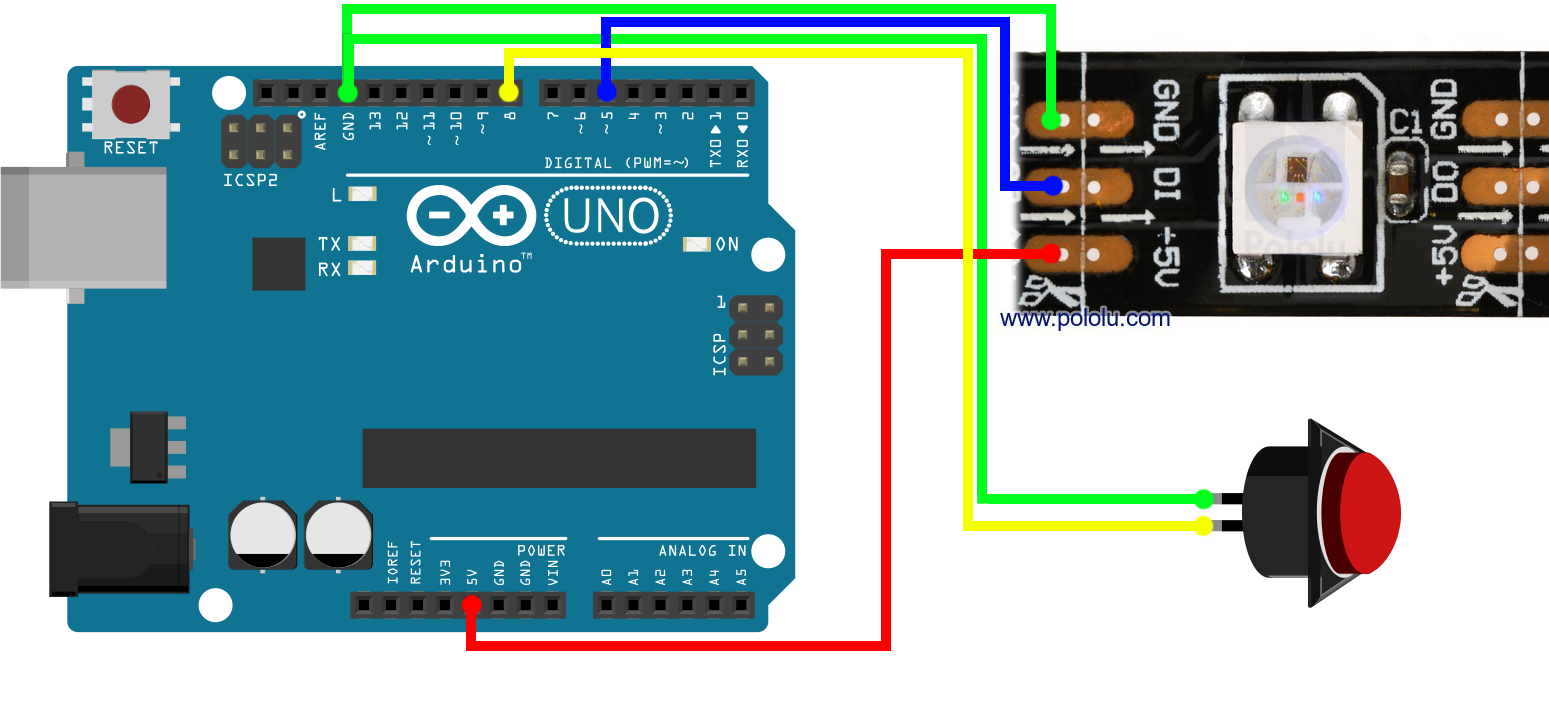
\includegraphics[scale=1]{img/schematic}
    \caption{Žaidimo komponentų sujungimo schema}
    \label{img:schema}
  \end{figure}

\section{Žaidimo veikimas}

  Žaidimas susideda iš mygtyko(vartotojo įvestis) ir ekrano(žaidimo būsena).
  Ekranas sudarytas iš 56 LED - 7 stulpeliai ir 8 eilutės.
  Žaidimo tikslas yra pastatyti bokštą.
  Žaidimas prasideda pirmame aukšte. Šviesos diodai juda pirmyn ir atgal pirmąjame aukšte.
  Šviesos diodai sudaro bloką sudarytą iš trijų diodų. Žaidėjui paspaudus mygtyką blokas
  pakeičia spalvą ir yra įrašomas atmintyje. Judantis šviesos diodų blokas yra perkeliamas vienu
  aukštu į viršų. Nuo antrojo aukšto žaidėjas prasideda žaidimo esmė. Žaidėjas turi
  pataikyti paspausti ant mygtuko taip, kad naujai atsiradęs šviesos diodų blokas,
  kuris juda pirmyn ir atgal dabartiniame aukšte, atitiktų vienu aukštu žemesnio išsaugoto bloko padėtį.
  Kitais žodžiais turi statyti tiesų bokštą. Jeigu žaidėjui nepavyksta visiškai pataikyti
  ant prieštai išsaugoto bloko žaidimas baigiamas - žaidėjas pralaimėjo. Bet kadangi diodų blokas sudarytas
  iš trijų diodų žaidėjas gali šiek tiek suklysi, bet tie diodai po kuriais nėra išsaugoto bloko bus prarasti
  ir vėlesniuose aukštuose pirmyn ir atgal judės ne trijų diodų blokas,
  o tiek diodų kiek žaidėjui pavyko pataikyti.

  Kad žaidimas netaptų per daug paprastas žaidžiant daug kartų kiekvienas papildomas aukštas
  pagreitina šviesos diodų bloko „vaikščiojimą“ pirmyn ir atgal. Taip pat kiekvienas naujas aukštas
  atsitiktinai parenka iš kurios pusės blokas pradės „vaikščioti“.

  \begin{figure}[H]
    \centering
    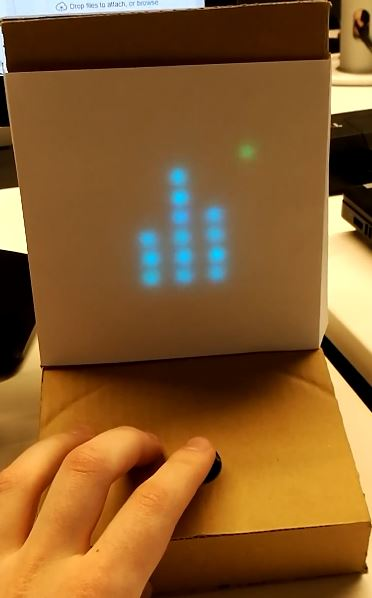
\includegraphics[scale=0.7]{img/game}
    \caption{Žaidimas}
    \label{img:game}
  \end{figure}


\section{Problemos}

  Kuriant žaidimą buvo susidurta su keleta problemų.

  \subsection{Litavimas}
    Kadangi litavimu nebuvo tekę užsiimti, o detalės yra smulkios ir trapios, lituoti buvo iššūkis.
    Norint iš LED juostos padaryti matricą teko juostą karpyti ir sujungti galus laidais.
    Litavimui naudotas lituoklis nebuvo ypatingas, o ir lituotojas ne ką geresnis.
    Dėl to sujungti sukarpytas LED juostos dalis buvo labai sunku ir teko daug kartų sulituoti,
    pabandyti įjungti ir pamatyti, jog prijungta nauja juostos dalis neveikia. Tada tekdavo bandyti atlituoti
    ir bandyti lituoti per naują.


  \subsection{Mygtukas}
    Pirmą kartą įjungus mygtuką pasirodė, jog viskas veikia gerai. Nes buvo tokia pavyzdinė programa,
    kurią užkrovus į Arduino ir paspaudus mygtuką LED lemputė turėtų užsigesinti.
    Bet pamodifikavus kodą, kad mygtukas veiktų atvirkščiai - paspaudus LED uždegamas, atleidus užgesinamas,
    mygtukas pradėjo neveikti ir lemputė pradėjo veikti tik kartais.
    Teko pasiskaityti internete, kodėl taip vyksta. Radau, jog reikia naudoti tam reikalui išvengti skirtą
    rezistorių - „pull-up resistor“. Arduino leidžia tokį rėžimą ijungti ant norimų kaiščių.


\sectionnonum{Rezultatai ir išvados}

  \subsection{Rezultatai}
    \begin{enumerate}
      \item Sukonstruotas žaidimo prototipas;
      \item Parašytas žaidimo programinis kodas.
    \end{enumerate}

  \subsection{Išvados}
    \begin{enumerate}
      \item Žaidimas veikia gerai, kaip ir tikėtasi;
      \item Žaidimą galima butų patobulinti, pridėti nesibaigiančio(endless) žaidimo rėžimą,
            aiškiau parodyti, kurioje vietoje žaidėjas suklyto, pakeisti sudetingumo(greičio) pridėjimo
            algoritmą bei pridėti skylę monetoms;
      \item Kūrimo proceso metu buvo įgyta daug naudingos patirties, kuri ateityje leis panašius pro-
            jektus atlikti geriau bei greičiau ir padės išvengti panašių problemų;
    \end{enumerate}


\appendix  % Priedai
% Prieduose gali būti pateikiama pagalbinė, ypač darbo autoriaus savarankiškai
% parengta, medžiaga. Savarankiški priedai gali būti pateikiami ir
% kompaktiniame diske. Priedai taip pat numeruojami ir vadinami. Darbo tekstas
% su priedais susiejamas nuorodomis.

\end{document}
